% --------------------------------------------------------------
% This is all preamble stuff that you don't have to worry about.
% Head down to where it says "Start here"
% --------------------------------------------------------------
 
\documentclass[20pt]{article}
 
\usepackage[margin=1in]{geometry} 
\usepackage{amsmath,amsthm,amssymb}
 
\newcommand{\N}{\mathbb{N}}
\newcommand{\Z}{\mathbb{Z}}
 
\newenvironment{theorem}[2][Theorem]{\begin{trivlist}
\item[\hskip \labelsep {\bfseries #1}\hskip \labelsep {\bfseries #2.}]}{\end{trivlist}}
\newenvironment{lemma}[2][Lemma]{\begin{trivlist}
\item[\hskip \labelsep {\bfseries #1}\hskip \labelsep {\bfseries #2.}]}{\end{trivlist}}
\newenvironment{exercise}[2][Exercise]{\begin{trivlist}
\item[\hskip \labelsep {\bfseries #1}\hskip \labelsep {\bfseries #2.}]}{\end{trivlist}}
\newenvironment{problem}[2][Problem]{\begin{trivlist}
\item[\hskip \labelsep {\bfseries #1}\hskip \labelsep {\bfseries #2.}]}{\end{trivlist}}
\newenvironment{question}[2][Question]{\begin{trivlist}
\item[\hskip \labelsep {\bfseries #1}\hskip \labelsep {\bfseries #2.}]}{\end{trivlist}}
\newenvironment{corollary}[2][Corollary]{\begin{trivlist}
\item[\hskip \labelsep {\bfseries #1}\hskip \labelsep {\bfseries #2.}]}{\end{trivlist}}

\newenvironment{solution}{\begin{proof}[Solution]}{\end{proof}}
\usepackage{graphicx}
\usepackage{natbib}
\usepackage[utf8]{inputenc}

 
\begin{document}
\title{Topic 3}
\author{Derek W Blackmon\\
Final Case Study:\\
Effects of Urban Development}

\maketitle







\renewcommand*\contentsname{\underline{TABLE OF CONTENTS}}

\newpage

\tableofcontents
\thispagestyle{empty}
\setcounter{page}{0}

\setlength{\parindent}{0cm}

\flushleft
\newpage

\section {Introduction}
As urbanization continues to present issues for future planning scenarios in the United States (U.S.), the necessity for persistent studies in urbanization and recommendations to policy makers will be necessary to mitigate potential losses of natural resources and green spaces. Further exasperating the issues of urbanization are scenarios in which urban sprawl does not take place in already vacant lots within an area but instead moves to an undeveloped area. Several case studies in North Carolina have indicated a 200 percent growth in localized areas population, resulting in 14-28 percent loss of timber resources (Dorning, et al., 2015). For the final case study, I will be examining and correlating articles I have researched in the past two months as well as incorporating new ideas, resulting in a better understanding of the issues surrounding urbanization. Figure 1 represents an infill development study (defined on page 5) taking place in Denver, Colorado and will be the focus of the final case study. Multiple scenarios and criteria had to be examined and considered for the Figure 1 map to be created. . 

\section{Literature Review}
Modelling land use change is critical to the understanding of the effects or urbanization scenarios. No perfect model or concept to demonstrate the impacts urbanization exists, but multiple studies throughout the United States using new technology and newly developed models seek to expand on what is already known. A study centered on the southeastern United States (U.S.) sought to demonstrate the impacts of urbanization and crop demand on habitat fragmentation and the implications to the wildlife caught in the middle of it all. Econometric modelling and wildlife species data were coupled together to create a predictive analysis of impacts of future land use changes on wildlife. The case study results showed tradeoffs of four scenarios, of which one scenario resulted in a 50 percent decrmpacts of urbanization.\\ 

\vspace{5mm} As mentioned earlier, studies conducted in North Carolina (N.C.) demonstrated the importance of natural resources. Urbanization can drastically impact the volume of timber available to the forest product industry in North Carolina, as well as employment in the state. There is an anticipation of as much as a 14 percent loss of forested areas in North Carolina by 2032 (Dorning, et al., 2015). A GIS was utilized to predict loss of forestland, based on a status quo growth scenario over study areas in N.C., resulting in predicative analysis of over 200 percent growth in developed areas in the study area (Dorning, et al., 2015). Coupling the potential loss of forest land with the impact on the regional economy creates yet another issue. The natural resource industry is a leading contributor to the economy throughout the U.S. but more specifically to the state of N.C., where natural resources contribute over 29 billion dollars annually (North Carolina Forest Service, 2017). As urbanization pressures increase the loss of natural resources it is likely to cause a decrease in economic productivity of regional areas dependent on forest products. The potential for habitat and economic loss are driving factors in continued education and policy implementation at the regional level to mitigate the effects of urbanization.\\   
\vspace{5mm} Not only are there habitat and natural resource/economic losses, but urbanization plays a role in societal issues. Frazier’s study on impacts of a shrinking city and associated crime statistics demonstrated an increase in crime given abandoned buildings and vacant areas *(Frazier, 2013). The importance of societal factors coupled with urbanization can lead to increasing rates of crime throughout cities. Given choices to leave areas abandoned in a city or utilize the abandoned space for development is an important thought process in planning for development. Another in depth case study involving urbanization and diffusion of crime demonstrated the interconnectedness of neighborhoods and crime issues *(Papachristos, 2018). When determining whether to fill in undeveloped areas of a city or not, crime rates in those areas will have to be considered, otherwise placing new developments in high crime areas will likely result in fewer people finding those areas suitable to live in. Habitat and economic loss and inclusion crime statistics can aid in the urban planning scenarios. In the end, knowing the audience is key to understanding how to develop a better solution to lessen effects of urbanization. Some regions of the U.S. may value more open space than others, or value being closer to amenities, which is why it is important to know who the product intends on representing.
\section{Case Study}
Figure 1, below, displays areas in Denver, Colorado most suitable for development using the Infill scenario. This map is the focus of my case study and my goals are to discuss the map, data used, and implications of the product. Figure 1 was created as a potential solution to reduce urban sprawl in the city of Denver. The project was created by college students from Tufts University, Massachusetts. Over 4,500 vacant/underutilized parcels were identified as being suitable for infill development (Kelly, 2017). Research this semester has shown the Infill scenario being one of several other scenarios considered for urbanization possibilities. The other scenarios have typically been, status quo, development exclusion, development constraint, and increased density. These scenarios are associated with Future Urban-Regional Environment Simulation (FUTURES) modeling. This type of model is composed of three sub-models (DEMAND, POTENTIAL, and PGA) to articulate future sites suitable for development. Using this approach can allow for inclusion of what is important to people, areas to preserve, as well as predict how much land will be needed for future development (Dorning, et al., 2015).
\begin{figure}[htp]
\centering
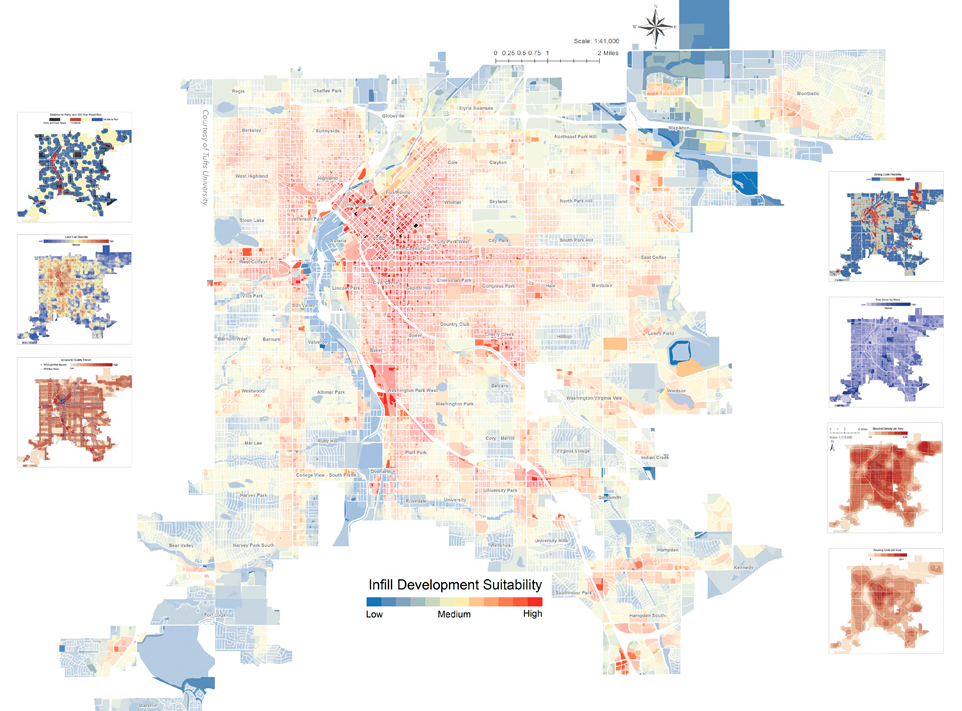
\includegraphics[width=\textwidth]{Figure 1.png}
\caption{Figure 1. Kelly, S., (2017). Analyzing Infill Development Suitability in Denver. ESRI Map Book, Volume 33, Planning and Engineering Section.}
\label{fig:Development Sustainability}
\end{figure}



\newpage
\begin{thebibliography}{1}

A GIS Code of Ethics. (2018). Retrieved February 13, 2019, from https://www.gisci.org/Ethics/CodeofEthics.aspx

\vspace{5mm}\newline Dorning, M. A., Koch, J., Shoemaker, D. A., and Meentemeyer, R. K. (2015). Simulating urbanization scenarios reveals tradeoffs between conservation planning strategies. Landscape and Urban Planning, 136, 28-39 
\vspace{5mm}\newline Esnard, A. M. (1998). Cities, GIS, and ethics. Journal of Urban Technology, 5(3), 33-45.
\vspace{5mm}\newline *Frazier, A. E., Bagchi-Sen, S., and Knight, J. (2013). The spatio-temporal impacts of demolition land use policy and crime in a shrinking city. Applied Geography, 41, 55-64.
\vspace{5mm}\newline *Joseph, B., Ping, N., Kurtis, Z., and Asia, T. (2018). Mapping urbanization in the United States from 2001 to 2011. Applied geography.
\vspace{5mm}\newline Kelly, S., (2017). Analyzing Infill Development Suitability in Denver. ESRI Map Book, Volume 33, Planning and Engineering Section.



\end{thebibliography}{1}




 
% --------------------------------------------------------------
%     You don't have to mess with anything below this line.
% --------------------------------------------------------------
 
\end{document}
